\chapter{Application in VAHSS}
\label{ch:VAHSS}
In this chapter, an application of the aggregated set membership proof is presented and evaluated. As discussed in chapter \ref{ch:intro}, VAHSS is an example where multiple data providers, henceforth denoted clients, participate. In this chapter first a construction of VAHSS  that verifies the servers computation is presented, then it is derived how to extend the verification to also include the clients. 
%The verification of clients requires each client to prove that the shared secret is in a predetermined allowed set or range.
Then different methods for verifying clients are compared. The comparison   mainly focuses on comparing aggregated signature-based set membership proof presented in Construction \ref{alg:ZKSM-Agg} with the state-of-the-art Bulletproofs for verification of clients to see how the runtime of the construction is affected.


\section{VAHSS}
\label{sec:VAHSS-HSS}
%Consider $n$ clients and $m$ servers, to simplify notation define the two sets $\mathcal{N}=\{1,...,n\}$ and $\mathcal{M} = \{1,...,m\}$. Let $c_i$ and $x_i$ for $i\in\mathcal{N}$ denote the clients (data providers) and their respective data. Denote the servers by $s_j$, where $\:j\in\mathcal{M}$.
The considered construction of VAHSS presented in \cite{SumItUp}, implemented and benchmarked in \cite{VAHSS}, makes use of homomorphic hash functions to verify the computations performed by servers.

%In this section the construction of the Verifiable Additive Homomorphic Secret Sharing (VAHSS), that this paper aim to extend is presented. The goal is to extend the VAHSS such that it in addition to  the verification of servers computations client are also verified to be honest. This will be done  by verifying that they do not provide false data. Different methods for verifying the data provided by the clients is explained in the next section.

%Before extending the VAHSS construction to additionally verify clients and combining it with the aggregated set membership proof introduced in the previous chapters. The VAHSS construction considered will be explained briefly. 

Assume that $n$ clients and $m$ servers participate in the VAHSS construction. The sets $\mathcal{N}=\{1,...,n\}$ and $\mathcal{M} = \{1,...,m\}$ are introduced to simplify notation. The clients are denoted $c_i$ for $i\in\mathcal{N}$, and their respective data $x_i$.  The servers in the construction are refereed to $s_j$ for $\:j\in\mathcal{M}$. 

Each client $c_i$ splits the secret $x_i$ into $m$ shares, denoted $\{x_{ij}\}_{j\in\mathcal{M}}$, such that $x_i=\sum_{j\in\mathcal{M}}x_{ij}$ and sends one share to each server. Each server $s_j$,  $j\in\mathcal{M}$, receives shares from all $n$ clients and computes and publishes the partial sum $y_j = \sum_{i\in\mathcal{N}} x_{ij} $. Then the final sum can be computed by any party by summing the public partial sums, which gives $y = \sum_{j\in\mathcal{M}} y_j = \sum_{j\in\mathcal{M}} \sum_{i\in\mathcal{N}} x_{ij} = \sum_{i\in\mathcal{N}} \sum_{j\in\mathcal{M}} x_{ij} =   \sum_{i\in\mathcal{N}}x_i$.

%For AHSS constructions, the idea is that each client splits their secret, $x_i$, into $m$ shares, denoted $x_{ij}$. The clients then sends one share to each server. The servers receives shares from all $n$ clients and computes the partial sum $y_j = \sum_{i\in\mathcal{N}} x_{ij} $ and publishes the result. The final sum can then be computed by any party by summing the public partial sums, this gives $y = \sum_{j\in\mathcal{M}} y_j = \sum_{j\in\mathcal{M}} \sum_{i\in\mathcal{N}} x_{ij} =  \sum_{i\in\mathcal{N}}x_i$. For VHASS construction in addition to AHSS a proof $\sigma$ that verifies that the partial sums $y_j=  \sum_{i=1}^n  x_{ij} $,  for all $j\in\mathcal{M}$, is generated and published. This allows any party to verify the correctness of the servers computations.

A proof $\sigma$ of the servers computations is obtained accordingly.  Each client $c_i$ publishes a checksum $\tau_i= g^{x_i+R_i}$, where $x_i$ is the secret hidden by the distributed shares and $R_i\in_R\mathds{F}$ is such that $R_n=\phi(p) \lceil \frac{\sum_{i=1}^{n-1}R_i}{\phi(p)}\rceil - \sum_{i=1}^{n-1}R_i $. Each server $s_j$ computes a partial proof $\sigma_j = g^{y_j}$.  Finally the verification is done by checking if $\prod_{j\in\mathcal{M}} \sigma_j = \prod_{i\in\mathcal{N}}\tau_i\wedge \prod_{i\in\mathcal{N}}\tau_i = g^y$.  If it holds the servers computations are proved to be correct. For a precise implementation and proof of correctness, security and verification the reader is refereed to the original paper about VAHSS \cite{SumItUp}.


\section{Client and Server VAHSS}
The VAHSS construction discussed in section \ref{sec:VAHSS-HSS} assumes honest clients and verifies the servers. This section extends the VAHSS construction to verify both the clients' input and the computations performed by the servers. First it is stated how to extend the VAHSS construction to additionally verify clients. Then a construction, using range proofs or set membership proofs, to verify clients is derived. It is then discussed how such a construction can be modified to use aggregated set membership proofs for verification of client' inputs. 

%If a range proof or set membership proof is included in the VAHSS construction then a potentially malicious clients can have a limited influence on the computed sum. Range proofs and set membership proofs force malicious input to still be part of a certain range or set. This leads to that the impact on the sum that a malicious client can have is bounded by the size of the range or by the elements in the set. 

% \subsection*{Verification of clients in VAHSS}
%In this section investigates how to combine the VHASS construction with a range proofs or set membership proofs.  Only range proofs and set membership proofs emanate from a Pedersen commitment hiding a secret is considered. 

\subsection*{Extending VAHSS to verify clients}
To ensure honest clients it is not sufficient to construct and perform a set membership proof and a VAHSS scheme separately. In such a protocol the verifier cannot be sure that the secret proven to be in the allowed set is the same as the secret hidden by the shares. The same principle holds considering range proofs. Therefore, a connection between the shares generated in the algorithm \textbf{ShareSecret} in the VAHSS construction and the secret hidden in a Pedersen commitment is desired. Proving that the sum of the shares is equal to the secret in a Pedersen commitment and then proving that the secret in the Pedersen commitment is in an allowed range or set convinces the verifier that the shares represent a secret that is in the allowed range or set. %The proof of the secret in the commitment is assumed to be a zero-knowledge range proof or zero-knowledge set membership proof of a secret in a Pedersen commitment.
%TODO fix: want to say general onlly
%Using the Pedersen commitment to link the VAHSS construction with a range proof or set membership proof, results in a general construction of a client and server VAHSS, compatible with any range proof or set membership proof of a secret in a Pedersen commitment.
% It is investigated if a Pedersen commitment can be included in the VAHSS construction, to obtain such a general construction of a client and server VAHSS 

%Publishing a Pedersen commitment of the secret itself does not provide any guarantee that it is the same secret that is hidden by the shares. It can also be seen that committing to the shares in Pedersen commitments does not ensure the verifier that the secret hidden in the shares are in the allowed set or range. This is since the individual shares themselves does not reveal information about the secret they are hiding. This leads to that there is not guarantee that proving a share belongs to the allowed range (or set) implies that the secret does and the other way assuming that the secret to a range (or set) does not imply that the shares does.

%Thus some trick to connect the secret in the shares to the secret in the Pedersen commitment must be derived. Therefore  that the aggregation of the partial proofs used in the VAHSS construction to prove the honesty of the servers will be used to connect the range proofs to the VAHSS construction.

In the VAHSS construction the clients publishes, in addition to the shares,  the checksums $\tau_i$ for the secrets $x_i$. Recall that the definition of the checksum is  $\tau_i=g^{x_i+R_i}$. %The checksum $\tau_i$ can be interpreted as a Pedersen commitment, where $g=h$.
Hereafter, the clients compute and outputs the Pedersen commitments $\pi_i=g^{x_i}h^{R_i}$, instead of the previously computed checksums $\tau_i$.  Given a commitment $\pi_i$, the clients can construct a range proof or set membership proof of the committed secret. It remains to argue that this would ensure the verifier that the secret hidden by the shares is the same secret proved to be in the allowed range or set as for all $i\in\mathcal{N}$.


%Therefore the  checksum may be used as a Pedersen commitment in the construction of a range proof  or set membership proof. Formally the checksum is a Pedersen commitment where $g=h$. However if $g=h$ the computationally binding property of a Pedersen commitment would not hold since $log_g(h)=log_g(g)=1$ which leads to that the left hand side in equation \eqref{eq:pedersen_binidng} is equal to $1$. Therefore to construct two commits $\mathds{E}(x,R)$ and $\mathds{E}(x',R')$ such that $\mathds{E}(x,R) = \mathds{E}(x',R')$ but $x\neq x'$ it is sufficient to solve solve for $x'$ in, 
%\begin{align*}
%R'-R = x-x'\:mod \:p .
%\end{align*}
%In other words it is straightforward to create a false commitment hence also a false range proof and set membership proof.

%TODO use set instead of range och fixa
Assume that client $c_k$ commits to the value $\hat{x}_k$ in the Pedersen commitment $\pi_k$, constructs the shares $\{x_{kj}\}_{j\in\mathcal{M}}$ such that $x_k = \sum_{j\in\mathcal{M}}x_{kj} \neq \hat{x}_k$ and  generates a ZKP that $\hat{x}_k$ belongs to the set $\Phi$ or range $[a,b]$. Since $x_k\neq\hat{x}_k$ this does not necessarily imply that  the secret hidden by the shares belongs to the range or set. Then  $\prod_{i=1}^m \pi_i \neq g^y$  and thereby the verification of servers does not succeed. Thus it has to hold that $x_k= \hat{x}_k$ for the protocol to succeed and any cheating client is detected. It is not possible to determine which party cheated and more precisely not even if the cheating party was a client or a server. 

\begin{Remark}
\label{thm:VAHSS_RP_CSV}
\vspace{10pt}
The correctness, security and verifiability requirements of a VAHSS construction holds after replacing the checksums $\tau_i= g^{x_i+R_i}$ with a Pedersen commitment $\pi_i= g^{x_i}h^{R_i}$ in the VAHSS construction, \cite{SumItUp}. 

Additionally if a range proof or set membership proof, denoted $\Sigma_i$, that satisfies the soundness, completeness and zero-knowledge requirements of zero-knowledge proofs is constructed of the secret $x_i$ in the Pedersen commitment $\pi_i$, for all clients $c_i$ in the VAHSS construction. Then any PPT adversary $\mathcal{A}$ who can modify the Pedersen commitments $\pi_i$  to any $\pi_i^{'} \:\forall  i\in T$, where $T$ is the set of corrupted clients, has a negligible probability of choosing a commitment $\pi_i^{'}$ such that verification of all the proofs $\Sigma_i$ and the VAHSS validates true.
%\begin{itemize}
 %\item \textbf{Verifiability Servers}  Let $\mathcal{A}$ denote any PPT  adversary and $T$ denote the set of corrupted servers with $T\leq m$. Note that if $|T|=m$, the verifiability property holds but not the security property. The verifiability property requires that any $\mathcal{A}$ who can modify the input shares to all servers $s_j\in T$ can cause a wrong value to be excepted as $y=f(x_1,...,x_n)$ with negligible probability.  
 %\item  \textbf{Verifiability Clients} 
%\end{itemize} 
\end{Remark}
%TODO fix proof before hand in to Seminar 2
\textbf{Proof of remark:}
The remark follows from that  replacing  $\tau_i$ with $\pi_i$ for $i=1,...,n$, it still holds that:
\begin{align*}
&\prod_{i\in\mathcal{N}} \pi_i = \prod_{i\in\mathcal{N}} g^{x_i}h^{R_i} = g^{\sum_{i\in\mathcal{N}} x_i}h^{\sum_{i\in\mathcal{N}} R_i} = g^{y} h^{ \phi(N)\big\lceil \frac{\sum_{i=1}^{n-1}R_i}{\phi(N) }\big\rceil} = g^y \\
&\text{Thereby it follows that: } \prod_{i\in\mathcal{N}}^n \tau_i = \prod_{i\in\mathcal{N}} \pi_i.
\end{align*}
Further the Pedersen commitment is perfectly hiding as well as computationally binding and thus it follows that the requirements are still fulfilled. 

From the soundness of range proofs and set membership proofs, and the above argument that the secret hidden in the commitment $\pi_i$ must be the same as the secret obtained by combining the the shares $\{x_{ij}\}_{j\in\mathcal{M}}$ for all $i=\mathcal{N}$, it follows that any adversary who can modify the commitments $\pi_i$ has a negligible probability of doing so such that the proofs $\Sigma_i$ and the VAHSS construction validates true. $\quad \square$

\begin{comment}
The correctness follows from the correctness of range proofs and by proving that $\sigma= \prod_{i=1}^n \pi_i \:\bigwedge\: \prod_{i=1}^n \pi_i = \mathcal{H}(y)$. Both $y$ and $\sigma$ are the same as in Construction \ref{alg:VAHSS-HSS}, hence by construction:
\begin{align}
    \label{eq:y=sum(x_ij)}
    y = \sum_{j=1}^m y_j= \sum_{j=1}^m \sum_{i=1}^n \lambda_{ij}p_i(\theta_{ij}) = \sum_{i=1}^n \overbrace{ \Big (\sum_{j=1}^m \lambda_{ij}p_i(\theta_{ij}) \Big)}^{ p_i(0)} = \sum_{i=1}^n p_i(0) = \sum_{i=1}^n x_i,
\end{align}
and for $\sigma$ it holds that:
\begin{align*}
    \sigma = \prod_{j=1}^m \sigma_j = \prod_{j=1}^m g^{y_j} = g^{\sum_{j=1}^my_j} =g^y = \mathcal{H}(y)
\end{align*}
For the $\pi_i$, whose construction has been modified compared to $\tau_i$ in  Construction\ref{alg:VAHSS-HSS}, thus it follows that:
\begin{align*}
    &\prod_{i=1}^n \pi_i = \prod_{i=1}^n \mathds{E}(x_i,R_i)= \prod_{i=1}^n g^{x_i}h^{R_i} = g^{\sum_{i=1}^n x_i } h^{\sum_{i=1}^n R_i} \overset{\eqref{eq:y=sum(x_ij)}}{=} g^y h^{\sum_{i=1}^{n-1} R_i+R_n} = \\ 
    &= g^y h^{ \phi(N)\big\lceil \frac{\sum_{i=1}^{n-1}R_i}{\phi(N) }\big\rceil} = g^y = \mathcal{H}(y) 
\end{align*}

The proof of security argument for malicious servers given in \cite{SumItUp} is still sufficient since the Pedersen commitment is perfectly hiding and computationally binding and that the range proofs are zero-knowledge. The security argument for malicious clients follows from the soundness of the range proof and that the secret hidden in the commitment has to be the same as the secret in the shares, as argued above. . 

The proof of \textit{\textbf{Verifiability Severs}} is the same as the proof given in  in \cite{SumItUp}, except that the commitments $\pi_i$ replaces the checksums $\tau_i$.  \textit{\textbf{Verifiability Clients}} follows from the properties of the range proof.
\end{comment}
%\end{proof}

\subsection*{Verifying clients using set membership proofs or range proofs}
A VAHSS where clients are verified by publishing range proofs or set membership proofs is presented in Construction \ref{alg:VAHSS-HSS-RP}.  In order to clarify the changes made to extend the construction to  verify clients, the differences to the VAHSS construction presented in \cite{SumItUp} are pointed out.

The algorithms \textbf{ShareSecret} and \textbf{Verify} has been modified,  and the algorithms \textbf{ProveSecret} and \textbf{GenerateCommitment} have been added. More precisely, the algorithm \textbf{ShareSecret} does not output the checksum $\tau_i$, instead the Pedersen commitment $\pi_i$ is computed in the algorithm \textbf{GenerateCommitment}. The algorithm \textbf{ProveSecret} constructs a set membership proof or range proof denoted $\Sigma_i$ given the commitment $\pi_i$. 
%The precise construction of the range proof or set membership proof that is used does not affect the rest of Construction \ref{alg:VAHSS-HSS-RP}, as long as it originates from a Pedersen commitment.
 In addition to the steps of the algorithm \textbf{Verify} in the VAHSS construction presented in \cite{SumItUp}, the algorithm \textbf{Verify} also validates the proofs $\Sigma_i$ for all $i\in\mathcal{N}$.
 
%The algorithm  \textbf{GenerateCommitment} can be included in either \textbf{ShareSecret}  or \textbf{RangeProof} instead of being viewed as a separate algorithm. In the implementation discussed later the commitment is generated while constructing the range proof and not explicitly. 

The algorithms \textbf{GenerateCommitment} and \textbf{ProveSecret} are executed by the clients and the other algorithms are executed by the same party as in the  VAHSS construction in \cite{SumItUp}. 

Remark \ref{thm:VAHSS_RP_CSV}  implies that Construction \ref{alg:VAHSS-HSS-RP} satisfies the correctness, security and verification requirements for a VAHSS construction and that the verification of clients' input satisfies the completeness, soundness and zero-knowledge requirements of the considered range proofs or set membership proofs.

%In the VAHSS Construction \ref{alg:VAHSS-HSS} the verifiability property includes verification of the servers. In this section this will be extended to also include the clients. The value $\pi_i$ published by the clients will be modified into a Pedersen commitment on the form $\pi_i = g^{x_i}h^{R_i}$, remember $\pi_i=g^{x_i+R_i}$ in the original construction presented in \cite{SumItUp}. The clients will apart from the previous commitments  also construct and publish a range proof for $\pi_i$. This allows any verifier to apart from verifying the servers also verify that the secret shared by the clients is in an certain range.  

%Given this construction the correctness, security and verification requirements for the server verifiable AHSS presented in \cite{SumItUp} is still fulfilled  that should be fulfilled is redefined below.  The difference to the requirements for the server verifiable AHSS is that additional demands for the clients behaviour is included. 

\begin{comment}
\begin{itemize}
    \item \textbf{Correctness} It must hold that Pr$\Big[\textbf{Verify}(\{\pi_i\}_{i\in\mathcal{N}},\sigma,y,\{\Sigma_i\}_{i\in\mathcal{N}})=1\Big]=1$. This means that with probability $1$ the output $y$ from \textbf{FinalEval} is accepted given all parties (clients and servers) where honest and the protocol were executed correctly.
    \item \textbf{Security} 
    			\begin{itemize}
    						\item \textbf{Malicious Servers } The construction should satisfy the same security argument as the VAHSS-HSS construction in \cite{SumItUp}.
    						%Let $T$ define the set of corrupted servers such that $|T|<m$, i.e at 					least one server is honest.  										Denote a PPT adversary by $\mathcal{A}_1$ and let the Adv$(1^			\lambda,\mathcal{A},T):= \text{Pr}[b' = b]-1/2$ be the advantage 										of $\mathcal{A}=\{\mathcal{A}_1,\mathcal{D}\}$ in guessing $b$ in the following experiment:
    							%		\begin{enumerate}
       						%				 \item The adversary $\mathcal{A}_1$ gives $(i,x_i,x_i')$ to the challenger, where $i\in[n], x_i\neq x_i'$ and $|x_i|=|x_i'|$.
        						%				\item The challenger picks a bit $b\in\{0,1\}$ uniformly at random chooses and computes $\textbf{ShareSecret}(1^\lambda,i,																\hat{x}_i) = (\hat{\text{share}}_{i1},...,\hat{\text{share}}_{im},\tau_i)$, where $\hat{\textbf{x}}_i$ is  such that $\hat{x}_i = 																\begin{cases}x_i, \text{ if } b=0 \\ x_i' \text{ else} \end{cases}$. 
        					%					\item Given the shares from the corrupted servers T and $\hat{\tau}_i$ the adversary distinguisger outputs a guess 																			$b'\xleftarrow[]{}\mathcal{D}((\hat{\text{share}_{ij}})_{j|s_j\in T},\hat{\tau}_i)$.
   									% \end{enumerate}
    							%		A VAHSS-construction is $t$-secure if for all $T\subset \{s_1,...,s_m\}$ with $|T|<t$ it holds that Adv$(1^\lambda,\mathcal{A},T)<												\varepsilon(\lambda)$ for some negligible $\varepsilon(\lambda)$.
  					  \item \textbf{Malicious Clients}  Since the construction does not clarify the exact range proof used, the security argument is refereed to the original papers for the used range proof and by proving that the secret hidden by the Pedersen commitments is the same as the secrets in the shares. 
   		 \end{itemize} 
 	\item \textbf{Verifiability} 
 			\begin{itemize}
 						\item \textbf{Verify Servers }Let $\mathcal{A}$ denote any PPT  adversary and $T$ denote the set of corrupted servers with $T\leq m$. The verifiability 							property requires that any $\mathcal{A}$ who can modify the input shares to all servers $s_j\in T$ can cause a wrong value to be excepted as 							$y=f(x_1,...,x_n)$ with negligible probability.   
 						\item \textbf{Verify Clients} Let $\mathcal{A}$ denote any PPT adversary and $T$ denote the set of corrupted clients. The verifiability property requires that any $\mathcal{A}$ who can modify the Pedersen commitments $\pi_i$  to any $\pi_i^{'} \:\forall  i\in T$ has a negligible probability at choosing a commitment $\pi_i^{'}$ such that Verify$( \{\pi^{'}_i\}_{i\in\mathcal{N}},x,y)=1$.
 			\end{itemize} 
\end{itemize}
\end{comment}

\begin{algorithm}
\caption{\textbf{: Client and Server Verifiable additive homomorphic secret sharing}}

\textbf{Goal:} Compute the sum $y = \sum_{i=1}^n x_i$. The values $x_i$ are kept secret. The servers computations and the clients shared values are verified. 
\vspace{2pt}\hrule\vspace{2pt}
\begin{itemize}
 \item\textbf{ShareSecret $(1^\lambda,i,x_i) \mapsto \{x_{ij}\}_{j\in\mathcal{M}}$} \\
Pick uniformly at random the coefficients, $\{a_i\}_{i\in\{1,..,t\}}\in_R\mathds{F}$ and define a $t$-degree polynomial $p_i$ to be on the form $p_i(X) = x_i + a_1X+...+a_tX^t$. Put the shares $x_{ij}=\lambda_{ij}p_i(\theta_{ij})$ for $j\in\mathcal{M}$.  The parameters $\theta_{ij}$ and Lagrange coefficients $\lambda_{ij}$ are chosen such that $ p_i(0) = \sum_{j=1}^m \lambda_{ij}p_i(\theta_{ij})$.
Output $\{x_{ij}\}_{j\in\mathcal{M}}$.

\item\textbf{GenereteCommitment$(1^\lambda,i,x_i) \mapsto \pi_i$ }\\
Let $R_i\in\mathds{F}$ be the output of a PRF such that $R_n\in \mathds{F}$  satisfies $R_n = \phi(N)\lceil \frac{\sum_{i=1}^{n-1}R_i}{\phi(N)}\rceil- \sum_{i=1}^{n-1}R_i $. Compute and output $\pi_i = \mathds{E}(x_i,R_i)= g^{x_i}h^{R_i}$.

\item\textbf{ProveSecret $(pp,x_i,\pi_i) \mapsto \Sigma_i$}\\
Construct a range proof or set membership proof, denoted $\Sigma_i$, for the Pedersen commitment $\pi_i$ of the secret $x_i$, on the  range $[a,b]$ or a set $\Phi$. All required public parameters, $pp$, needed to  construct the proof $\Sigma_i$ is assumed to be pre-shared and known by all parties.
\item\textbf{PartialEval $(j,\{x_{ij}\}_{i\in\mathcal{N}})\xrightarrow[]{}y_j$}\\
Compute and output $y_j = \sum_{i=1}^n x_{ij}$.

\item\textbf{PartialProof $(j,\{x_{ij}\}_{i\in\mathcal{N}})\xrightarrow[]{}\sigma_j$}\\
Compute and output $\sigma_j = \prod_{i=1}^n g^{x_{ij}} =  g^{\sum_{i=1}^n x_{ij}}= g^{y_j}=\mathcal{H}_1(y_j)$.

\item\textbf{FinalEval $(\{y_j\}_{j\in\mathcal{M}})\xrightarrow[]{}y$}\\
Compute and output $y = \sum_{j=1}^m y_{j}$.

\item\textbf{FinalProof $(\{\sigma_j\}_{j\in\mathcal{M}})\xrightarrow[]{}\sigma$}\\
Compute and output $\sigma = \prod_{j=1}^m \sigma_j = \prod_{j=1}^m g^{y_{j}} =  g^{\sum_{j=1}^m y_{j}}= g^{y}=\mathcal{H}_1(y)$.

\item\textbf{Verify $(\{\pi_i\}_{i\in\mathcal{N}},x,y,\{\Sigma_i\}_{i\in\mathcal{N}})\xrightarrow[]{}\{0,1\}$}\\
Compute and output $\sigma= \prod_{i=1}^n \pi_i \wedge \prod_{i=1}^n \pi_i = \mathcal{H}_1(y)\wedge \{\textbf{VerifyProof}( \Sigma_i) \}_{i\in\mathcal{N}}$. $\textbf{VerifyProof}$ is the verification algorithm of  the  proofs $\{\Sigma_i\}_{i\in\mathcal{N}}$.
\end{itemize}
\label{alg:VAHSS-HSS-RP}
\end{algorithm}

\subsection*{Verifying clients using aggregated set membership proofs}
Construction \ref{alg:VAHSS-HSS-RP-Agg} describes a client and server VAHSS compatible with aggregated set membership proofs for verification of clients. The algorithms in Construction \ref{alg:VAHSS-HSS-RP-Agg} are the same as in Construction \ref{alg:VAHSS-HSS-RP} except that the algorithm \textbf{PartialAggregate} is introduced and the algorithm \textbf{Verify} is modified. 

The algorithm \textbf{PartialAggregate} is run by all aggregating parties in the set $\mathcal{K}$ and the algorithm \textbf{Verify} is modified such that it verifies the aggregated proofs instead of the individual clients' proofs.

If the server computing the partial sums $y_j$ are responsible for aggregation of the clients set membership proofs, then no new parties are introduced to the VAHSS construction to aggregate the proofs.  Then the set $\mathcal{K}$ is equal to $\mathcal{M}$ in construction \ref{alg:VAHSS-HSS-RP-Agg}. 
 
For aggregation in Construction \ref{alg:VAHSS-HSS-RP-Agg} to be sound, the aggregation must either be performed by a trusted party or split between at least two aggregating parties. 

If the aggregation is performed by an untrusted party, this party can cheat in the aggregation of the proofs, by exploiting that the sum $y$ can be computed once the servers have performed the algorithm \textbf{PartialEval} and that  $h^{\sum_{i\in\mathcal{N}} R_i } =1 \: \text{mod}\:  \phi(p)$. Note that this induces that  the assumptions of Theorem \ref{thm:aggrgeation} are not fulfilled, since the aggregation party has additional knowledge beyond the input to the algorithm \textbf{Aggregate} and the commitments $\{C_i\}_{i\in\mathcal{S}}$. %Although the individual secrets are unknown, it is possible to cheat when constructing the aggregated proof $\Sigma_a$, by using the fact that $y=\sum_{i\in\mathcal{N}}x_i, h^{\sum_{i\in\mathcal{N}}R_i}$ are known. 
Since $y$ is known to the aggregating party, the aggregated proof $\Sigma_a$ can be constructed as, $D_a=C^{k+c}, z_{R_a} = k\phi (N)$ and $z_{x_a} = k y$, where $y= \sum_{i\in\mathcal{N}} x_i$ and $k\in_R \mathds{F}$. Then it follows that:
\begin{align*}
D_a &= C^{k+c}= \big( g^ { k \sum_{i=1}^n x_i } h^{ k  \sum_{i=1}^n R_i ) } \big)   \big( g^{ (  \prod_{i=1}^n c_i ) \sum_{i=1}^n x_i ) } h^{ ( \prod_{i=1}^n c_i ) \sum_{i=1}^n R_i ) } \big)   \\
 C^c h^{z_{R_a}}g^{z_{x_a}} &= C^c h^{k \phi (N) } g^{k y} =  \big( g^{ (  \prod_{i=1}^n c_i ) \sum_{i=1}^n x_i ) } h^{ ( \prod_{i=1}^n c_i ) \sum_{i=1}^n R_i ) } \big) h^{k\phi (N)} g^{ky}\\
= &  \big( g^{ (  \prod_{i=1}^n c_i ) \sum_{i=1}^n x_i ) } h^{ ( \prod_{i=1}^n c_i ) \sum_{i=1}^n R_i ) } \big)g^ { k y} h^{ k  \phi(N)\lceil \frac{\sum_{i=1}^{n-1}R_i}{\phi(N)}\rceil ) }\\
& \implies D_a = C^ch^{z_{R_a}}g^{z_{x_a}}.
\end{align*}

It has been shown that if one party aggregating all clients' set membership proofs the aggregation is not sound, since the aggregated proof can be constructed such that it validates true without proving the statement in equation \ref{eq:SMagg_statement}. 
%Further it is seen that  it is possible for such an aggregating party to  cheat and provide an aggregated proof that  verifies true without the statement in equation \eqref{eq:SM_statement} being true.

If multiple parties aggregates subsets of the proofs, the assumptions in Theorem \ref{thm:aggrgeation} holds,  this follows from that the sum of the secrets and random values are unknown considering any true subset of the clients. 

Under the assumption that the aggregation is sound, Remark \ref{thm:VAHSS_RP_CSV} applies to Construction \ref{alg:VAHSS-HSS-RP-Agg}. Thereby, if the aggregation is performed by a trusted party or is split between at least two independent aggregating parties, Construction \ref{alg:VAHSS-HSS-RP-Agg} satisfies the correctness, security and verification requirements for a VAHSS construction and the verification of clients' input satisfies the completeness, soundness and zero-knowledge requirements of the considered range proofs or set membership proofs. 

\begin{algorithm}
\caption{\textbf{: Client and Server Verifiable additive homomorphic secret sharing}}

\textbf{Goal:} Compute the sum $y = \sum_{i=1}^n x_i$. The values $x_i$ are kept secret. Servers computations and clients shared values are verified. 
\vspace{2pt}\hrule\vspace{2pt}
\begin{itemize}
 \item\textbf{ShareSecret $(1^\lambda,i,x_i) \mapsto \{x_{ij}\}_{j\in\mathcal{M}}$} \\
Pick uniformly at random the coefficients, $\{a_i\}_{i\in\{1,..,t\}}\in_R\mathds{F}$ and define a $t$-degree polynomial $p_i$ to be on the form $p_i(X) = x_i + a_1X+...+a_tX^t$. Put the shares $x_{ij}=\lambda_{ij}p_i(\theta_{ij})$ for $j\in\mathcal{M}$.  The parameters $\theta_{ij}$ and Lagrange coefficients $\lambda_{ij}$ are chosen such that $ p_i(0) = \sum_{j=1}^m \lambda_{ij}p_i(\theta_{ij})$.
Output $\{x_{ij}\}_{j\in\mathcal{M}}$.

\item\textbf{GenereteCommitment$(1^\lambda,i,x_i) \mapsto \pi_i$ }\\
Let $R_i\in\mathds{F}$ be the output of a PRF such that $R_n\in \mathds{F}$  satisfies $R_n = \phi(N)\lceil \frac{\sum_{i=1}^{n-1}R_i}{\phi(N)}\rceil- \sum_{i=1}^{n-1}R_i $. Compute and output $\pi_i = \mathds{E}(x_i,R_i)= g^{x_i}h^{R_i}$.

\item\textbf{ProveSecret $(pp,x_i,\pi_i) \mapsto \Sigma_i$}\\
Construct a range proof or set membership proof, denoted $\Sigma_i$, for the Pedersen commitment $\pi_i$ of the secret $x_i$, on the  range $[a,b]$ or a set $\Phi$. All required public parameters, $pp$, needed to  construct the proof $\Sigma_i$ is assumed to be pre-shared and known by all parties.
\item\textbf{PartialEval $(j,\{x_{ij}\}_{i\in\mathcal{N}})\xrightarrow[]{}y_j$}\\
Compute and output $y_j = \sum_{i=1}^n x_{ij}$.

\item\textbf{PartialProof $(j,\{x_{ij}\}_{i\in\mathcal{N}})\xrightarrow[]{}\sigma_j$}\\
Compute and output $\sigma_j = \prod_{i=1}^n g^{x_{ij}} =  g^{\sum_{i=1}^n x_{ij}}= g^{y_j}=\mathcal{H}_1(y_j)$.

\item \text{\textbf{PartialAggregate} $(pp,k,\mathcal{S}_k, \{\Sigma_i\}_{i\in\mathcal{S}_k} ) \xrightarrow[]{} \Sigma_{a_k}$} \\
On the input $\{ \Sigma_i \}_{i\in\mathcal{S}_k}$ where $\mathcal{S}_k\subseteq\{1,...,n\}$, the set of proofs is aggregated according to the algorithm \textbf{Aggregate} in Construction \ref{alg:ZKSM-Agg} and  aggregated proof $\Sigma_{a_k}$ is published. 

\item\textbf{FinalEval $(\{y_j\}_{j\in\mathcal{M}})\xrightarrow[]{}y$}\\
Compute and output $y = \sum_{j=1}^m y_{j}$.

\item\textbf{FinalProof $(\{\sigma_j\}_{j\in\mathcal{M}})\xrightarrow[]{}\sigma$}\\
Compute and output $\sigma = \prod_{j=1}^m \sigma_j = \prod_{j=1}^m g^{y_{j}} =  g^{\sum_{j=1}^m y_{j}}= g^{y}=H(y)$.

\item\text{ \textbf{Verify} $(\{\pi_i\}_{i\in\mathcal{N}},x,y,\{\Sigma_{a_k} \}_{k\in\mathcal{K}})\xrightarrow[]{}\{0,1\}$}\\
Compute and output $\sigma= \prod_{i=1}^n \pi_i \wedge \prod_{i=1}^n \pi_i = H(y)\wedge \{\textbf{VerifyProof}(\Sigma_{a_k})\}_{k\in\mathcal{K}}$. $\textbf{VerifyProof}$ is the verification algorithm in Construction \ref{alg:ZKSM-Agg}.
\end{itemize}
\label{alg:VAHSS-HSS-RP-Agg}
\end{algorithm}


%For the VAHSS construction this can be implemented by letting the server, which computes the partial sums, aggregate different subset of the clients set membership proofs. 

 %And if the set set of aggregating parties $\mathcal{K}$ consist of one element and $\mathcal{S}_k  = \mathcal{N}$ the partial aggregation would correspond to a full aggregation, and Construction \ref{alg:VAHSS-HSS-RP-Agg} would describe the aggregated client and severs VAHSS construction for a single trusted aggregating party. 

%To conclude, if the aggregation is not assumed to be performed by a trusted party then the characteristics of the VAHSS construction all set membership proof cannot be aggregated by a single party. Thus then the aggregation must the split between atleast two parties.  


%The main result obtained is that it is possible to extend the VAHSS construction presented in Construction \ref{alg:VAHSS-HSS} such that honesty of the clients is verified. The proposed verification of clients ensure the verifier that all clients shared secrets belonging to a pre-specified allowed range or set. Given the existence of such a range or set, each client provides a zero-knowledge proof that their secret is in the range or set. The verification algorithm for the client and sever verifiable AHSS, compared to the algorithm in Construction \ref{alg:VAHSS-HSS}, is extended to verify all range proof or set membership proofs published by the clients. This leads to that the verifier after having performed the verification is convinced that all secrets in the summation belongs to the allowed range or set, and that all servers computations was done correctly. 

%All constructions examined to provide a proof that a secret is in an allowed range or set, assumes that there exists pre-published Pedersen commitment of the secret and proves the statement for the secret in the commitment.  Exploiting this similarity between various range proofs and set membership proofs when combining them with a VAHSS lead to that a general methodology for including verification of clients in the VAHSS construction. The proposed client and server VAHSS in Construction \ref{alg:VAHSS-HSS-RP} is independent of the construction used to prove that a statement in in an allowed range or set, given that it is proved for a secret in a Pedersen commitment. Note that it is implicitly assumed that 
%construction can provide a proof for the desired range or set and that
%the algorithm for construction of the proof and verifying of the proof are compatible.

%Theorem \ref{thm:VAHSS_RP_CSV} states the correctness, security and verification of Construction \ref{alg:VAHSS-HSS-RP}. It is seen that the extending the VHASS with a verification of the clients preserves the correctness, security and verification requires for the VAHSS. Moreover the verifier is convinced that the secrets shared by the clients belongs to an allowed range or set. 


\section{Implementation}
\label{sec:implementation}
%TODO what to include here? 
% Discuss translation to Golang. 
An implementation of Constructions \ref{alg:VAHSS-HSS-RP} and \ref{alg:VAHSS-HSS-RP-Agg} is obtained to investigate the proposed clients and server VAHSS in a practical setting and comparing the runtime for different methods for verifying clients.
%To provide an implementation of Construction \ref{alg:VAHSS-HSS-RP} and \ref{alg:VAHSS-HSS-RP-Agg} the algorithms constructing a VAHSS  are combined with the algorithms to prove and verify clients.  Bulletproofs, aggregated and not aggregated signature-based set membership proofs are the considered methods for verifying clients.  %is provided written in Golang. 

%Remark that this construction is written without specifying which range proof that is used, and works for all different range proofs that provides a proof for a Pedersen commitment, which is true for all range proof discussed above.
 %From the prototype analysis given above it is clear that Bulletproofs is faster than signature-based range proof. Considering the aggregation possibility for signature based range proofs, Construction \ref{alg:VAHSS-HSS-RP} will be implemented using all three considered proofs to ensure honest clients. 
 
%  all three constructions will hence be used to implement the client and server verifiable additive homomorphic secret sharing construction \ref{alg:VAHSS-HSS-RP}. 

Bulletproofs, aggregated and non-aggregated signature-based set membership proofs implemented in Golang are publically available on Github, \cite{Git:RP} \cite{Git:mycode}. The VAHSS construction implemented in both python and C++,  is available at \cite{Git:python_vahss} and \cite{Git:C_vahss} respectively. 

To implement Construction \ref{alg:VAHSS-HSS-RP} and \ref{alg:VAHSS-HSS-RP-Agg},  the VAHSS algorithms need to be callable from the same programs as the algorithms for Bulletproofs, signature-based set membership proofs and aggregated signature-based set membership proofs. The VAHSS algorithms have been translated to Golang, to solve the problem of having the implementations written in different programming languages. The implementation is available at \cite{Git:mycode}.

To provide an implementation of Construction \ref{alg:VAHSS-HSS-RP} and \ref{alg:VAHSS-HSS-RP-Agg} besides translating the VAHSS code to Golang the implementations have also been slightly modified. The VAHSS construction has as discussed above been adjusted such that it considers a Pedersen commitment $\pi_i$ instead of the checksum $\tau_i$. The implementations of Bulletproofs, signature-based set membership proofs and aggregated signature-based set membership proofs have also been adjusted to be compatible with the VAHSS algorithms. These adjustments are merely to merge the constructions and does not change the semantics of the constructions. The modified implementations are available at \cite{Git:mycode}.


% To achieve this one of the two following modifications needs to be done. The first alternative is to \texit{wrap} the code from one programming language such that it can be compiled and used by another programming language. This would then mean to either write a wrapper for Go code such that it can be interpreted by a C++ (or Python) compiler, or alternatively wrap the  CC++ (or Python) code such that it can be interpreted by a Go compiler. The second alternative is to translate the VAHSS implementation into the same language as the Bulletproofs, signature-based range proof and set membership proof or the other way around. 

%The first alternative appears to be a simpler approach hence this is first tested. In 2016 \textit{cgo} was released which enables calling C functions from Go code. 
%The Go command \textit{cgo} enables Go packages to call C code. TODO...

%Instead consider the second alternative, that translating the code of one of the implementations such that all code is available in the same programming language. Since the VAHSS construction is  shorter than the two range proofs and the set membership proof all together, the VAHSS code was converted to Go.


%Besides translating the VAHSS implementations to Go a small adjustments of the already existing Go implementations of the range proofs and set membership proof  had to be done to merge with the VAHSS construction. This adjustment are merely to merge the codes and does not change the semantics of the range proofs. What has been  modified is that the randomness used in the Pedersen commitments in the range proof must be chosen such that $R_n = \phi(N)\lceil \frac{\sum_{i=1}^{n-1}R_i}{\phi(N)}\rceil- \sum_{i=1}^{n-1}R_i$, hence is is regarded as input to the proof constructions.The full code for combination of range proofs (or set membership proofs) and VAHSS is available at Git \ref{Git:MyCode}. 

%Just as in construction \ref{alg:VAHSS-HSS-RP} the implementation of the code aims to be  general, such that all three concerned range proofs can be used to verify clients honesty and the merge of the range proof to the VAHSS construction is the same for all range proofs. However note that although the construction does not specify which range proof that is used the implementation does due o the choice of underlying group in the set up, the signature-based range proofs and set membership proof uses pairing friendly elliptic curve groups in the implementation which is not the case for Bulletproofs. This leads to minor modifications of the implementation to adapt to range proofs and set membership proofs.
\subsection*{Implementation parameters}
The finite field $\mathds{F}$ is generated by a prime of size $256$-bit.

The number of servers is set to $5$, $|\mathcal{M}|=5$,  and the number of clients to $100$, $|\mathcal{N}|=100$.  The set of aggregation parties $\mathcal{K}$ is assumed to consist of a single party, meaning that $|\mathcal{K}|=1$.

Remark that the trade-off between runtime for aggregation and verification depending on the number of aggregation parties is presented in section \ref{sec:tradeoff}.  The result presented there translates directly to the runtime of the aggregation and the verification of clients in a server and client VAHSS.  Thereby, although $|\mathcal{K}|=1$ in this section the runtime considering multiple aggregating parties can be obtained by studying the results presented in chapter \ref{ch:results}.

The range is set to $[18,200]$ for the implementation of Bulletproofs, and thus the upper bound of the Bulletproof is set to $2^n$, where $n=8$. The size of the set $\Phi$ is put to the length of the range, $|\Phi|=200-18 = 182$, for both the aggregated and not aggregated signature-based set membership proofs. 

A final remark about the implementation is that its purpose is to test the above-proposed constructions and provide runtime evaluations, the code has not been tested enough to be considered as a secure implementation.



% runtime is important
% not aggregation here 
%This paper has studied three different constructions possible to combine with a VAHSS to verify clients. In the runtime comparison of these three constrictions, seen in Table \ref{tab:runtime}, it was noted that the set membership and Bulletproofs where notable faster than the signature-based range proof. Further it has been discussed that the set membership proof can be used a larger area of applications. This is due to that it proves membership of a sets which are more flexile than ranges. 

%Although the discussion above is favourable towards Bulletproofs and set membership proofs,  Construction \ref{alg:VAHSS-HSS-RP} has be implemented considering Bulletproofs, set membership proofs and signature-based range proofs. The runtime is consequently presented for all three combinations. This is also motivated by completeness of the comparison. 

\section{Prototype analysis}
%The implementation of Constructions \ref{alg:VAHSS-HSS-RP} and \ref{alg:VAHSS-HSS-RP-Agg}, using different construction to verify clients, are benchmarked to provide runtime results. The runtime results are used to compare the different constructions for verifying clients.

%Combining the VAHSS with a verification of clients, as done in Construction \ref{alg:VAHSS-HSS-RP} and \ref{alg:VAHSS-HSS-RP-Agg}, resulted in a constructions where the VAHSS algorithms are run almost in parallel to the algorithms for a range proofs or set membership proofs. The interaction between the two constructions is minimal and appears only in the verification.  Consequently it can be expected that the runtime for the different algorithms in Construction \ref{alg:VAHSS-HSS-RP} and \ref{alg:VAHSS-HSS-RP-Agg} are almost the same as the runtime for the algorithms for them in individual constructions, i.e VAHSS and range proofs or set membership proofs.

%For example the algorithms  \textbf{ShareSecret}, \textbf{PartialEval} run completely independent of the algorithm \textbf{RangeProof} in Construction \ref{alg:VAHSS-HSS-RP} and \ref{alg:VAHSS-HSS-RP-Agg}, resulting in that they are almost identical to the algorithms in the original VAHSS construction, \cite{SumItUp}. Thus the runtime for the algorithms are likely to comparable with the results given in \cite{VAHSS}. The same hold the other way around, that the algorithm \textbf{RangeProof} is likely to be comparable to previous runtime results, \cite{RANGE-SET}. 

%Smaller adjustment has been made to the algorithms due to combining and hence the runtime for all algorithms in the  the client and server VAHSS in evaluated.  

The runtime for the algorithms in Construction \ref{alg:VAHSS-HSS-RP} and \ref{alg:VAHSS-HSS-RP-Agg} is presented in Table \ref{tab:BenchBP}. Construction \ref{alg:VAHSS-HSS-RP} is benchmarked considering two different constructions for verifying clients:  Bulletproofs and signature-based set membership proofs. Construction \ref{alg:VAHSS-HSS-RP-Agg} is benchmarked considering aggregated signature-based set membership proofs, with a single trusted aggregating party.
 


 %TODO use in discussion
%The results in the table confirms the previous perception that  signature-based range proofs are not competitive with Bulletproofs in runtime performance. In addition since Bulletproofs can also be used for arbitrary ranges, it is concluded that Bulletproofs are to prefer above signature-based range proofs. 


%Note that although the construction does not specify which range proof that is used the implementation does due o the choice of group in the set up, the signature-based range proofs and set membership proof uses pairing friendly elliptic curve groups in the implementation which is not the case for Bulletproofs.

In Construction \ref{alg:VAHSS-HSS-RP} and \ref{alg:VAHSS-HSS-RP-Agg} there is one algorithm called \textbf{Verify}, verifying both clients and servers.
To separately measure the runtime for verifying the servers and clients the  algorithm \textbf{Verify} is split into two procedures, \textbf{VerifyServers} and \textbf{VerifyClients}. The first procedure, \textbf{VerifyServers}, performs the verification of the servers computations. The second procedure  \textbf{VerifyClients}, verifies the clients by evaluating their range proofs or set membership proofs. To clearly state what the algorithms \textbf{VerifyServers} and \textbf{VerifyClients} correspond to, consider the following reformulation of the algorithm \textbf{Verify}: 
\begin{itemize}
 \item\textbf{Verify $(pp, \{\pi_i\}_{i\in\mathcal{N}},y,\{\Sigma_i\}_{i\in\mathcal{N}})\xrightarrow[]{}\{0,1\}$}\\
 Verify the clients and servers according to, 
 	\begin{itemize}
 	\item \textbf{VerifyServers $(\{\pi_i\}_{i\in\mathcal{N}},y)\xrightarrow[]{}\{0,1\})$}\\
 Compute and output $\sigma= \prod_{i=1}^n \pi_i \wedge \prod_{i=1}^n \pi_i = H(y)$.
 \item \textbf{VerifyClients $(\{\pi_i\}_{i\in\mathcal{N}}\{\Sigma_i\}_{i\in\mathcal{N}})\xrightarrow[]{}\{0,1\}$ }\\
 For each proof $\Sigma_i$, verify that it is correct. This implies running  $\textbf{VerifyProof}(\pi_i, \Sigma_i)$ for all $i\in\mathcal{N}$, where $\textbf{VerifyProof}$ is the verification algorithm associated with the algorithm used to construct the proof, $\Sigma_i$. If the proofs have been aggregated then the verification is performed for each aggregated proof instead of for each clients proofs. If all proofs are correct return $1$, else $0$.  
 \end{itemize}
Return  $\textbf{VerifyServers}\wedge \textbf{VerifyClients}$
\end{itemize}

 \begin{table}[h]
\centering
\caption{Runtime for the algorithms in Construction \ref{alg:VAHSS-HSS-RP} and \ref{alg:VAHSS-HSS-RP-Agg}. The runtime of Construction \ref{alg:VAHSS-HSS-RP} is presented using Bulletproofs and signature-based set membership proofs to verify clients.  Aggregated signature-based set membership proofs are used to verify clients in Construction \ref{alg:VAHSS-HSS-RP-Agg}}
\begin{tabular}{l  c c c}
\toprule
&   \multicolumn{2}{c}{\textbf{ Construction \ref{alg:VAHSS-HSS-RP}}}    &	\textbf{Construction \ref{alg:VAHSS-HSS-RP-Agg}}	\\ 
    																	& Bulletproofs  & Set membership & Aggregated Set membership\\	\midrule
  \textbf{GenerateShares}				  					&95 [$\mu$s]			 &98 [$\mu$s]  &98 [$\mu$s]												\\ 
  \textbf{ProveSecret} 						&53 [ms]				& 	66 [ms]	&66 [ms]			\\ 
  \textbf{PartialEval}  										&   78 [$\mu$s]				&71 [$\mu$s]	 		&	71	 [$\mu$s]							\\ 
  \textbf{PartialProof} 									&   273 [$\mu$s]						& 5255 [$\mu$s]			& 5255 [$\mu$s]				\\ 
   \textbf{Aggregate}										&   				&			&		59 [s]					\\ 
  \textbf{FinalEval}  											&   689 [ns]						&699  [ns]				&			699  [ns]												\\ 
  \textbf{FinalProof}  												&   50 [$\mu$s]			&  115 [$\mu$s]	&				115 [$\mu$s]									\\ 
  \textbf{VerifyClients}							  							&   2979 [ms]					& 9288 [ms]&					8120 [ms]							\\ 
  \textbf{VerifyServers}											&   1672 [$\mu$s]					&		7947 [$\mu$s] 	&		7947 [$\mu$s]					\\ 
  \bottomrule
\end{tabular}
\label{tab:BenchBP}
\end{table}
%Considering this paraphrase, it is clear what the runtime \textbf{VerifyServers} and \textbf{VerifyClients} in Table \ref{tab:BenchBP} measures. Note that \textbf{VerifyServers} is the runtime to verify all servers and \textbf{VerifyClients} is the runtime for verifying all client.

In Table \ref{tab:BenchBP} the runtime for all algorithms are  consistently faster when using Bulletproofs to verify the clients. Note that the considered range is $[18,200]$, hence it is sufficient to use $n=8$ for the upper bound for the Bulletproofs. In section \ref{sec:ComparetOBullet} it is noted that the runtime for verification of multiple clients increased significantly if the upper bound of the range is increased. This implies that if a larger range is considered the aggregated signature-based set membership would be faster than Bulletproofs for verification of all clients. This is seen in Chapter \ref{ch:results} in Figure \ref{fig:NrClients}. 

Uniformly, independent of which construction used to verify clients, the runtime for \textbf{VerifyServers} is approximately $10^3$ times faster than for \textbf{VerifyClients}.  This highlights how expensive the verification of clients is and motivates the attempt to reduce the computations required to verify multiple clients by aggregating set membership proofs. 

Considering the runtime of \textbf{VerifyClients}, it is noted that aggregation of signature-based set membership proofs reduce the runtime by $13\%$. The set membership proofs are only partly aggregated and thereby the runtime depends on the number of provers. Consequently, when a large number of clients participate the verification of clients still becomes a bottleneck of the construction.


It is noted that the algorithms \textbf{PartialProof}, \textbf{FinalProof} and \textbf{VerifyServers} differs noteworthy in runtime for different constructions for verifying clients. These algorithms, as described in Construction \ref{alg:VAHSS-HSS-RP} and \ref{alg:VAHSS-HSS-RP-Agg}, are seemingly independent of the construction used to verify clients. The  difference in runtime comes from that different libraries for the elliptic curve groups are used for Bulletproofs and the signature-based set membership proofs. %Optimisation of the libraries has not been made and whether the difference can be reduced due to optimisations is not investigated.
The libraries have not been benchmarked against each other, and whether the difference in runtime can be reduced via optimisations has not been investigated.

%The runtime  for the algorithms \textbf{PartialProof}, \textbf{FinalProof} and \textbf{VerifyServers} using Bulletproof for verification of client is not affected by increasing the maximum upper bound. I.e Bulletproofs are consequently, independent of implementation parameters, faster then aggregated signature-based set membership proofs, for these algorithms.

%Which construction of proving clients honesty to prefer depends on the applications. It has been discussed that the size of the range, which party that has lowest computational capacity and how many clients are in the construction are three important factors determining the suitability of different constructions. 

%TODO here or not? 
%The preference of which method to use for verification of clients is application specific. Determined by which party has the highest computational power and which party the lowest. 




%In Figure \ref{fig:NrClients} the runtime of \textbf{VerifyClients} is given as a function of the number of clients, for Bulletproofs and set membership proofs. This means that \textbf{VerifyRP} as defined above is ran $1,25,50,75,100,125$ respective $150$ times.  From the figure it is seen that the is a almost a linear relationship between the number of clients and the runtime. This is not surprising since the verifier has to perform the step \textbf{VerifyRP} once for each client. 

%The computational complexity of Bulletproofs depends on the maximal upper bound of the range. The maximal upper bound of Bulletproofs is $2^n$, for some $n$. 
%The computational complexity depends on $n$ and is $\mathcal{O}(log_2 n)$. 
%Up to this point it has been assumed that the range is $[18,200]$, thus it has been sufficient use the maximal upper bound $2^8=256$, i.e $n=8$.  If a different range were considered, then the upper bound might need to be altered. This motivates to see how the runtime is affected by considering an other upper bound. 

%By construction of Bulletproofs $n$ must a power of $2$, thus the runtime is tested for $n=32$.   More precisely the runtime for \textbf{VerifyClients} depending on the number of clients, as described above, is benchmarked for Bulletproofs with the maximal upper bound equal to $2^{32}$. This result is seen in Figure \ref{fig:NrClients}. Further it is noted that the runtime for Bulletproofs with a upper limit equal to $2^{32}$, the verification is slower than for set membership proofs. 


%TODO deside if use this, plus rerun all values!
% The Bulletproofs has computational complexity $\mathcal{O}(log_2 n)$, thus an expected increase of a factor $5/3\:(=log_2\: 32/ log_2\: 8)$ would be expected, however in Figure \ref{fig:NrClients} an increase of a factor approximately $4$ is seen for the algorithm \texttt{Verify} in Construction \ref{alg:VAHSS-HSS-RP} when increasing $n$ form $8$ to $32$, why this result is obtained is not clear.

% \begin{figure}[]
%\caption{Runtime for the verification of clients honesty depending on the number of clients. The runtime is compared between set membership proofs and two different instances of Bulletproofs,  maximal upper bound of the range is $2^8$ respective $2^{32}$ for the Bulletproofs instances.}
%\label{fig:NrClients}
%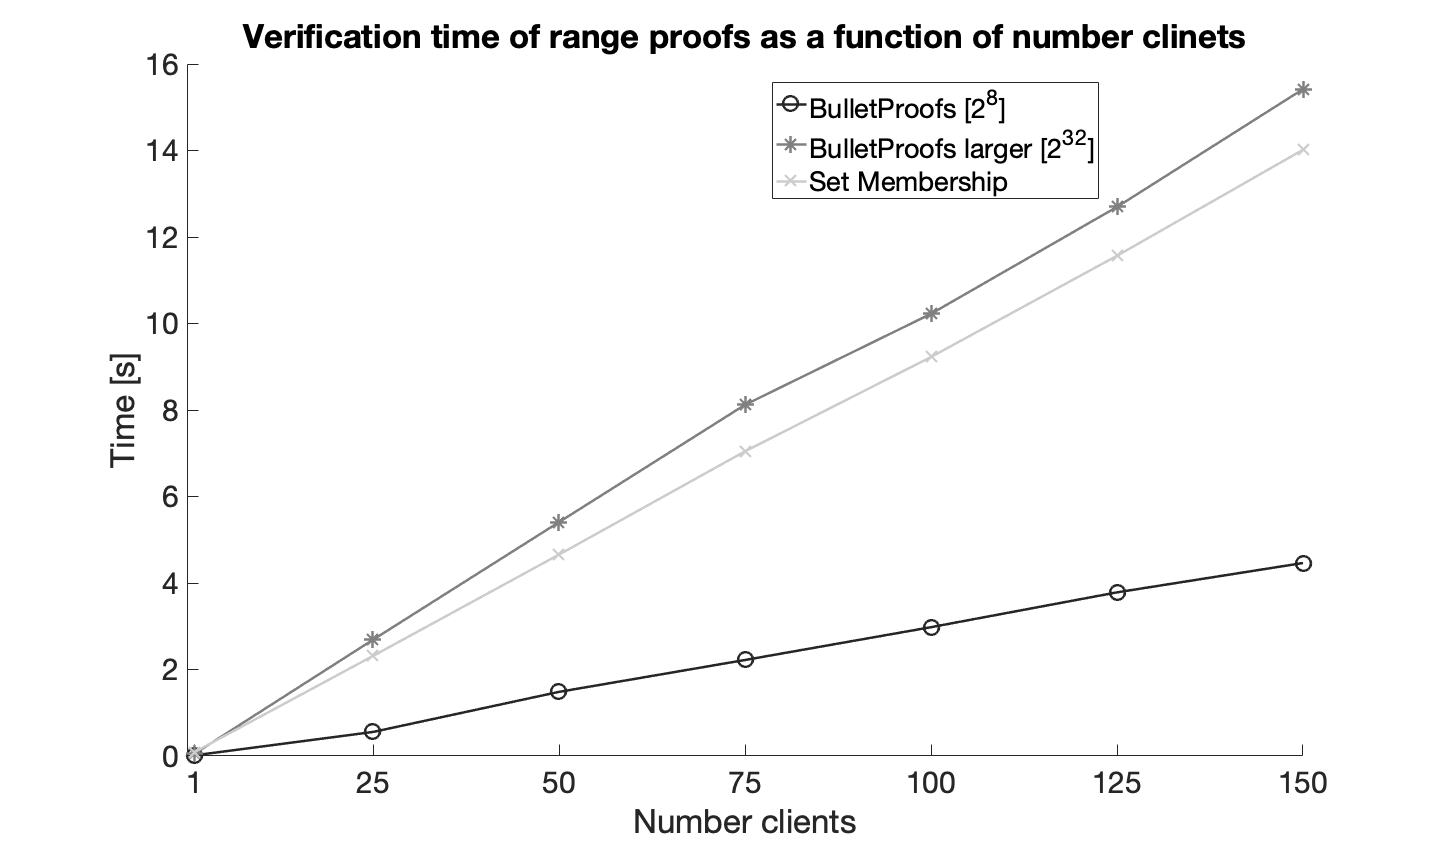
\includegraphics[width=\linewidth]{./figure/verification_nrClients.png}
%\end{figure}
